Humans have been modifying Earth’s ecosystems for thousands of years. Archaeological and palaeontological evidence suggest that human activities may have played a major role in the extinction of Australian’s megafauna as early as fifty thousand years ago \citep{Johnson2016, Miller2016, VanDerKaars2017}. 
The subsequent arrival of modern humans in other parts of the world has also been associated with extinctions, of the megafauna in particular \citep{Sandom2014, Broughton2018}. However, the global signature of human presence on Earth has never been as prominent as in recent decades. The past two hundred years have been characterised by a sharp increase in the rates of human-driven changes at the planetary scale, a phenomenon that has been termed `the Great Acceleration' \citep{Steffen2015}. To emphasize the recent impacts of human activities on the Earth’s systems, \citet{Crutzen2000} proposed that we have entered a new geological epoch, which they called `the Anthropocene'. Although the formal acceptance of this epoch and the timing of its start are still debated within the stratigraphic community \citep{Lewis2015, Monastersky2015}, the coined term reflects the profound effects of humans on planetary processes and on the biosphere, such that its use has largely surpassed the geological field \citep{Malhi2017}. 

The Anthropocene can be characterised by Earth-system and socio-economic indicators \citep{Steffen2011, Biermann2016}. Two of the major signatures are the human-driven transformations of the land surface, and changes to atmospheric composition, which have led to the onset of anthropogenic climate change \citep{Lewis2015}. Altogether, the development of human activities at unprecedented scales and magnitude has led to the alteration of many ecosystems. As a result of combined anthropogenic pressures, the world’s biodiversity has been changing \citep{Dirzo2014, McGill2015, Johnson2017, Daru2021}. 
Decreases in a range of biodiversity indicators have been reported for many taxonomic groups \citep{Butchart2010}. Human-mediated invasions and translocations of species, coupled with local declines in native species, have promoted biotic homogenisation \citep{Newbold2018a, Daru2021, FinderupNielsen2019}.
In addition, species have gone extinct at rates higher than expected from natural background variability, with current extinction rates estimated to exceed those inferred from fossil records by a hundred to a thousand times \citep{Barnosky2011,DeVos2015}. Biodiversity loss and ecosystem change have become such major issues in the 21\textsuperscript{st} century that the prevention of biodiversity erosion and the protection of ecosystems have become priority goals on international agendas \citep{Hoban2020, CBD2020}. Indeed, it is now well established that biodiversity is tightly linked with ecosystem functioning and ecosystem services delivery \citep{Oliver2015, Hooper2005, MA2005}, and thus ultimately with human well-being \citep{MA2005}. However, the difficulty in achieving global conservation goals – such as the failure to reach the Aichi targets \citep{Buchanan2020} – highlights the need to strengthen global conservation efforts if we are to protect biodiversity and related ecosystem services from global threats \citep{Butchart2016}. 

\section{Major drivers of global biodiversity change}

Currently, land-use change is the primary driver of global biodiversity loss, and is responsible for causing global declines in species richness and abundance through habitat modification \citep{Newbold2015, Chaudhary2018a, Nowakowski2018a, Powers2019, Maxwell2016}. Although climate change is not currently the main driver of biodiversity change, the negative effects of climate change on biodiversity could equate those of land-use change in their magnitude by 2070 \citep{Newbold2018}. Other major drivers of biodiversity loss include overexploitation, pollution and the spread of non-native species. In this thesis, my focus is on land-use and climate change as global drivers of biodiversity change.

\subsection{Land-use change}

Land cover describes the physical aspect and composition of the land surface from dominant biotic and abiotic features, typically classifying the Earth’s surface into determined sets of natural and artificial ensembles (e.g., grasslands, forests, man-made structures, waterbodies, etc; \citet{Grekousis2015}). Land cover can notably be characterised with satellite imagery \citep{Wulder2018}. Land use, however, describes the human intent behind a particular land cover \citep{Lambin2001}. Land-use change thus refers the process by which humans transform the landscape to achieve socio-economic needs. Land-use change includes transitions from natural to anthropogenic landscapes, as exemplified by agricultural-driven deforestation in tropical areas \citep{Jayathilake2021}. It also describes transitions between different forms of human-dominated land uses, such as the expansion of urban areas over agricultural lands \citep{Ustaoglu2017}. Land-use change can also include transitions from anthropogenic land uses to natural habitats, for example with the restoration of human-degraded landscapes \citep{BanksLeite2020}. Land-use and land-cover classifications may overlap, and these two terms have often been used interchangeably \citep{Comber2008}. Although humans have been modifying terrestrial ecosystems for millennia – between 75\% and 95\% of the total land surface could have been altered by human activities at some point in history  \citep{Ellis2013, Ellis2021} – it is only during the past three centuries that the terrestrial surface made the transition from mostly wild to mostly human-dominated \citep{Ellis2010}. The most important driver behind this transition has been agricultural expansion, with major increases in cropland and grazing areas from the mid-18\textsuperscript{th} century onward (Figure \ref{Introduction_fig1}a). In recent decades, the expansion of grazing areas and animal feed crops, fuelled by the rising demand for animal products, has been identified as the most important driver of land-use change \citep{Alexander2015}. 

The effects of land-use change on biodiversity have been characterised at local, regional and global scales – although global-scale studies represent a small proportion of the published research \citep{Davison2021}. Overall, land-use change  has a negative impact on species richness and abundance \citep{Newbold2015, Foley2005}. For example, urban areas, which have been expanding at faster rates than urban populations themselves \citep{Seto2010}, can have a considerable negative impact on biodiversity and ecosystem services, despite currently representing a small proportion of the terrestrial surface (about 1\%; \citet{Goldewijk2017}). In particular, the expansion of impervious surfaces, which characterizes urban development, has been linked to a reduction in species richness \citep{Souza2019, Yan2019} and to increases in environmental risks (e.g., due to flooding, \citet{Hou2022}; or to heat-island effects). Another important aspect of land-use change for biodiversity outcomes and ecosystem service delivery is the level of intensity at which the land is used to fulfil its purpose. For instance, management practices in agricultural areas are a major determinant of local biodiversity and related ecosystem services such as pollination and pest control \citep{Foley2005, Kehoe2015a, Millard2021}. In urban areas, introducing and managing green spaces can lead to positive biodiversity outcomes \citep{Ives2016, Aronson2017}, and can also help mitigate flooding risks and heat islands \citep{Livesley2016}. Yet, land-use intensity has not been explicitly considered by a majority of past studies investigating impacts of land-use change on biodiversity \citep{Davison2021, Dullinger2021}.

\begin{figure}[h!]
\centering
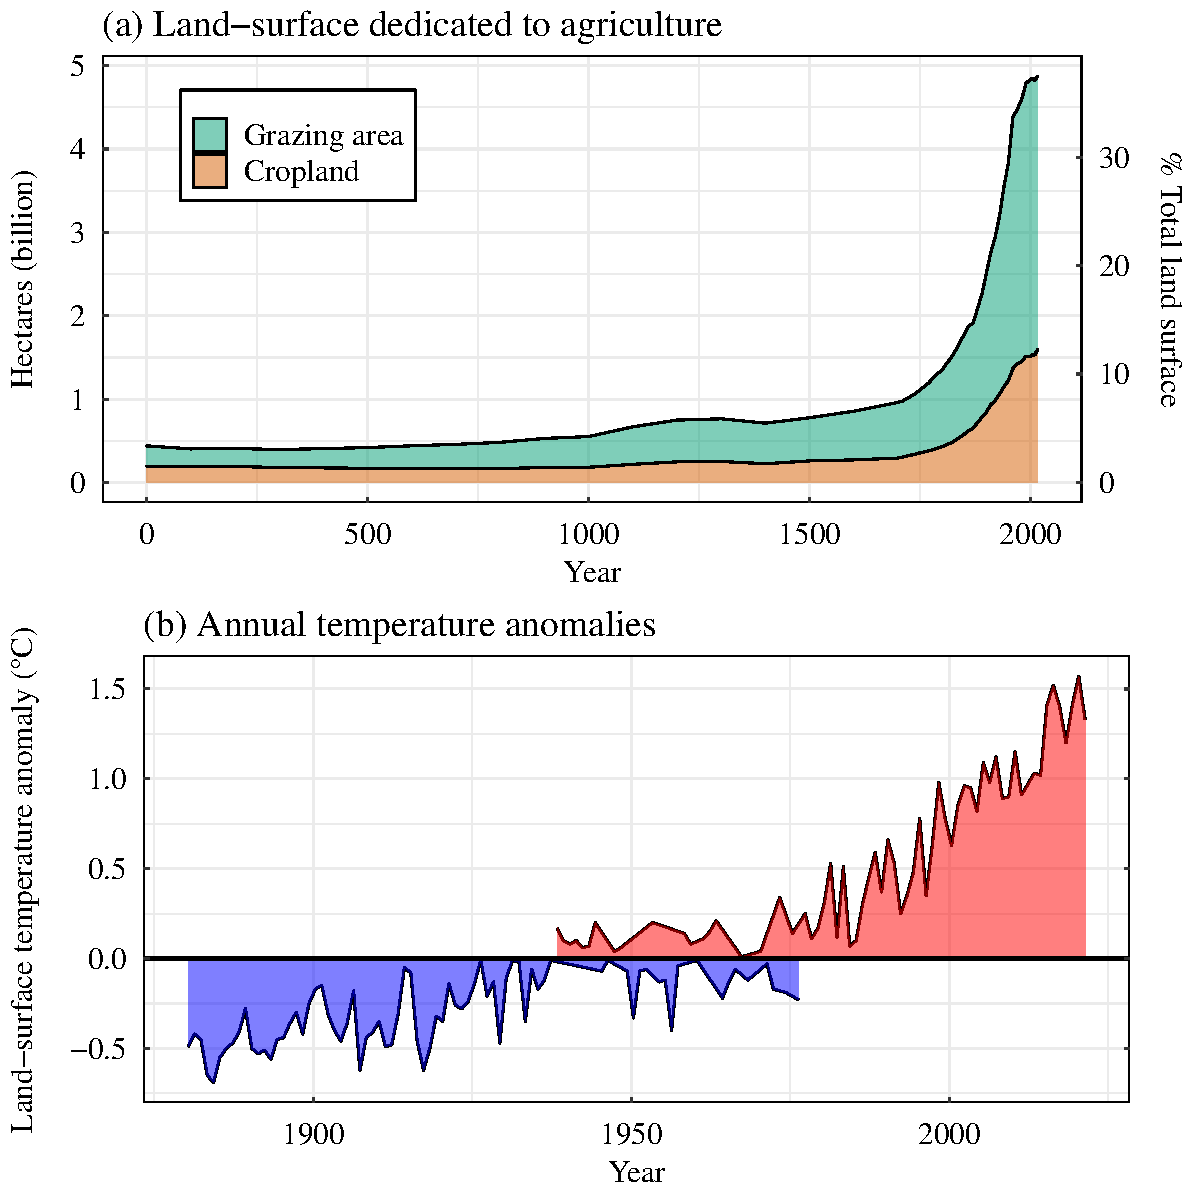
\includegraphics[scale=0.55]{figures/Chapter1/Intro_plot}
\caption[Characteristics of the `Great Acceleration']{\textbf{Characteristics of the `Great Acceleration'.} \textbf{(a)} Land surface (and \% land-surface) used for agricultural purposes between year 0 and 2016. Data from the HYDE database \citep{Goldewijk2017}, downloaded from \url{https://ourworldindata.org/land-use} (24/01/2022). \textbf{(b)} Annual land-surface temperature anomaly between 1880 and 2021. Data retrieved from the National Oceanic and Atmospheric Administration – National Centers for Environmental Information, Climate at a Glance: Global Time Series, published April 2022, retrieved 06/05/2022 from \url{https://www.ncdc.noaa.gov/cag/}. The anomalies are calculated with reference to the global temperature average for the 20\textsuperscript{th} century. }
\label{Introduction_fig1}
\end{figure}

\subsection{Climate change}

According to the World Meteorological Organization, climate change is defined as long-term changes (i.e, over at least several decades) to the mean state or to the variability of the climate, attributable to human activity or to natural causes. There is a strong scientific consensus that current climate change (from approximately 1850) is the result of human-driven changes to atmospheric composition \citep{Crowley2000, IPCC2013, Maibach2014}. Current manifestations of climate change include rising average temperatures (\citet{Valipour2021}; Figure \ref{Introduction_fig1}b), increases in the frequency of extreme events \citep{Seneviratne2012}, and changes in global rainfall patterns \citep{Dore2005, Trenberth2011}. 

There is accumulating empirical evidence that climate change affects biodiversity globally, with documented changes in phenology \citep{Inouye2022}, in the geographical distributions of species \citep{Chen2011, Lenoir2015, Soroye2020}, and in species physiology \citep{Portner2008, Chown2010}.  Climate-change impacts on individual species have consequences for whole communities, through disruptions of species interactions, which can in turn exacerbate impacts on individual species \citep{Cahill2013, Kharouba2018}. 


\subsection{The future of biodiversity in the Anthropocene}

Projecting future land-use and climate-change impacts on biodiversity highlights the key role of human-development scenarios for global biodiversity outcomes \citep{Newbold2018, Powell2013}, for the long-term viability of animal populations \citep{Spooner2018}, and for ecosystem processes and services \citep{Lawler2014}. As the world’s population continues to grow and as the demand for food, energy and other commodities keeps rising, rates of global land-use and climate change are unlikely to slow without the implementation of strong international regulations and consumption changes \citep{IPCC2022, Stehfest2019}. Under current development scenarios (`business as usual'), future projections show that biodiversity will likely be negatively impacted overall, with decreases in species abundance, increases in extinction rates, and shifts in the distribution of species \citep{Schipper2020, Pereira2010, Newbold2018}. In this context, evaluating the effects of land-use and climate change on biodiversity and associated ecosystem services has become vital in order to put into place mitigation measures. Understanding how species have responded to past and current pressures can help assess how they are likely to respond to future pressures. In particular, understanding what makes species more sensitive to land-use and climate change can help conservation efforts and mitigate global human impacts on biodiversity. 


\section{Ecological importance of terrestrial vertebrates and current threats}

In this thesis, I focus on terrestrial vertebrates, a group of more than 30,000 species that has been particularly well sampled and studied \citep{Titley2017}, and for which there is available ecological information for many species (such as geographical distributions, traits, occurrence, etc.), allowing for large-scale biodiversity assessments (e.g., \citet{Jenkins2013}). Terrestrial vertebrates  play significant roles in ecosystem functioning and support a wide range of processes, most notably as pollinators \citep{Ratto2018}, seed dispersers \citep{Tiffney2004}, regulators of lower trophic levels \citep{Barber2010, Salo2010, Luck2012, Lin2018, Zhang2018_trophicinter}, nutrient cyclers \citep{Wilson2011, Inger2016, Cunningham2018} and ecosystem engineers \citep{Severtsov2012}. Vertebrates are also important for human societies, both culturally and as sources of proteins \citep{Hirons2016, Albert2018, Alves2018}, and feature among the most charismatic species in the public’s eye \citep{Courchamp2018, Albert2018}.

Despite their cultural and ecological importance, terrestrial vertebrates are highly threatened by human activities. The latest Living Planet Report revealed that vertebrate populations have decreased by 70\% on average since 1970 \citep{WWF2020}. According to the IUCN Red List of Threatened Species, about 41\% of assessed amphibian species, 26\% of mammals, 21\% of reptiles and 13\% of birds are classified as threatened with extinction (IUCN 2022, \url{https://www.iucnredlist.org/resources/summary-statistics}). A recent assessment of vertebrates listed in the IUCN Red List of Threatened Species highlights habitat destruction as the predominant human threat \citep{Cox2022}, but direct exploitation also features among the major factors of decline \citep{Monastersky2014}. Although climate change is not the principal driver of current population declines \citep{Caro2022}, the first extinction of a mammal (the Bramble Cay melomys, \textit{Melomys rubicola}) attributed to anthropogenic climate was reported in 2016 \citep{Watson2016}. Future projections highlight that between 10\% and 30\% of vertebrate species could be locally lost by 2070 depending on climate-change scenarios \citep{Newbold2018}, and that up to one in six species could face extinction under current climate change \citep{Urban2015}. Further, despite having been well sampled and studied compared to other groups, there still remain important gaps and biases in our ecological knowledge of terrestrial vertebrates and of their responses to human threats \citep{Meyer2015, Meiri2016, Hevia2017, Oliver2021}.


\section{Using trait-based approaches to understand global biodiversity change}

\subsection{Traits as common currencies across species}

Despite the global average declines reported for vertebrate populations, not all species respond similarly to environmental changes \citep{Dornelas2019, Leung2020}: while some species are impacted negatively, others benefit from global environmental changes \citep{Thomas2013, Newbold2018a}. One of the reasons why species differ in their ability to cope with disturbances is that species present different characteristics, or traits. In my thesis, I use the term `traits' to refer to \textit{intrinsic} characteristics, i.e. measurable at the level of an individual. Thus, although the formal definition of a trait can vary depending on studies, I adopt the definition of \citet{McGill2006}, considering traits to be characteristics that are measurable at an organismal level, comparable across different species, and that likely influence organismal fitness and performance. I further make a distinction between `traits' and `ecological characteristics', notably in Chapter 4, where I refer to `ecological characteristics' as encompassing traits and geographical range area (as geographical range area does not meet the strict definition of a trait).

The idea that species traits mediate species' responses to environmental change was formalised in the `response-effect' framework, developed in the field of plant ecology \citep{Lavorel2002a}, where traits that influence species' responses to environmental change were termed `response traits' (and those that underpin ecological processes were termed `effect traits'). One of the appeals of trait-based approaches is that individual species are no longer the fundamental unit of biodiversity investigations. Rather, traits become the focus and act as `common currencies' across species, which is of particular interest for conservation when long-term population data are lacking. If species' responses to human threats consistently relate to certain traits, it may be possible to generalise patterns, and estimate the responses of species for which population data are not available \citep{Verberk2013}. 

\subsection{Using ecological traits to assess which species are at most risk from human-driven changes}

Vertebrate ecological traits (which I distinguish from physiological traits, and which I define here as traits relating to the life-history, diet, morphology, and habitat use of species) have been used to explain species' responses to global changes. Past studies have notably investigated whether species extinction risk is associated with species traits \citep{Lebreton2011, Ripple2017, Chichorro2019}, which is of high interest for conservation, but often lacks a consideration of specific threats \citep{GonzalezSuarez2013}. 

Other studies have focused on the influence of traits on species' responses to particular human pressures. For example, a range of correlative trait-based approaches have been used to understand whether traits are associated with species' responses to climate change. 
On the one hand, past work has made use of spatial data to investigate species' responses to climate change. For instance, some studies have focused on explaining interspecific variation in past or projected range shifts with traits \citep{Schloss2012, Mccain2014, Pacifici2017, DiMarco2021}. 
However, studying observed responses to climate change may be complicated by the fact that this requires disentangling the effects of climate change from effects of other drivers of change on observed responses \citep{MacLean2017}. Thus, other studies have used proxies instead of observed responses, which may provide complementary insights into the relationships between traits and species' ability to track climate change. For instance, \citet{Estrada2018} used a `range-filling' approach as a proxy for species' ability to shift their distributions under climate change. The `range-filling' approach consists of investigating interspecific differences between the realised and potentially suitable climatic niche of species, differences which are interpreted as being driven by intrinsic (i.e., traits) and/or extrinsic factors (e.g., non-climatic environmental factors, biotic interactions, etc.) limiting the realised distribution of the species \citep{Estrada2018, Svenning2004}. Intrisic factors found to constrain species' realised distribution could also limit species' ability to track climate change, and as such could confer higher climate-change sensitivity.
On the other hand, demographic approaches relying on long-term population data have also been employed to explain population- and species' responses to recent climate change \citep{Spooner2018}. These approaches may suffer from similar complications regarding the disentangling of climatic and non-climatic effects on observed responses \citep{Williams2022}. 
Finally, ecological traits have been used in a predictive fashion, notably with frameworks aiming to assess species' vulnerability to climate change \citep{Foden2013, Pacifici2015}, assuming that given traits confer higher sensitivity to climate change. 

Past studies have also investigated whether traits are associated with species' responses to habitat disturbance. Most of these studies have used spatial data, inferring effects of land-use change on biodiversity from `space-for-time' substitutions \citep{DePalma2018, Davison2021}, such as in \citet{Newbold2013}, \citet{Quesnelle2014} or \citet{Nowakowski2017}.

Further, trait-based approaches have also been employed to understand the signature of human impacts on the diversity and variability of traits within ecological communities. To this end, a range of functional diversity indices have been developed \citep{Schleuter2010a, Legras2018}. Functional diversity indices have been employed to evaluate the effects of land-use disturbance on the trait diversity of vertebrate assemblages (most often at local and regional scales; \citet{Flynn2009}; \citet{LaSorte2018}; \citet{Tinoco2018}), or to assess the projected effects of climate change on the trait diversity of vertebrate species \citep{Stewart2022}.

Although trait-based approaches using ecological traits have been widely employed to understand the effects of human-driven changes on vertebrate species, past studies have mostly been conducted at local to regional scales \citep{Davison2021}, and have tended to focus on given taxa among the vertebrate classes \citep{Hevia2017}. Thus, global comparative assessments of the relationships between ecological traits and species' responses to human pressures across terrestrial vertebrates are lacking. Because of the diversity of approaches used to investigate associations between species traits and human pressures in past work, and because of the different spatial scales and taxonomic focus of past studies, identifying a set of traits that emerge as important determinants of sensitivity to both land-use and climate change across terrestrial vertebrates remains challenging. For instance, \citet{Quesnelle2014} found that reproductive rates, as estimated from litter or clutch sizes, were significantly associated with sensitivity to habitat loss in wetland vertebrates; however, \citet{Nowakowski2017} did not find any effect of clutch size on amphibian sensitivity to habitat modification. The meta-analysis by \citet{MacLean2017} highlights the lack of consensus in published studies on the associations between traits and species' range shifts on under recent climate change.
Thus, there remains a need to assess whether and which traits are associated with species' responses to human pressures in terrestrial vertebrates. 

\subsection{Using physiological traits to understand  land-use impacts on biodiversity and ecosystem functioning}

Physiological traits are typically measured to capture aspects of species' metabolism, performance or biochemistry. Recent decades have seen advances in large-scale studies linking physiological traits to macroecological patterns of species existence across levels of organisation \citep{Chown2004, Burger2021}, as exemplified by the development of the `metabolic theory of ecology' \citep{Gillooly2001a, Brown2004a}. In particular, metabolic rates reflect the amount of energy used at the organismal level (I define metabolic rates here as the rates at which an organism processes available energy, which is often measured in the lab by estimating the amount of consumed O\textsubscript{2} by a whole organism over a period of time \citep{Sadowska2015, Auer2017}). As energy is a fundamental currency across all living organisms, metabolic rates can be employed comparatively across species to investigate interspecific variation in energetic expenditure. Thus, past studies have focused on understanding intraspecific variation in metabolic rates \citep{Burton2011, Auer2017} as well as interspecific variation (such as variation in metabolic rates with temperature; \citet{Clarke2004a}; or variation in metabolic rates with longevity -- e.g., testing the `pace of life' theory; \citet{Stark2020}).

How species allocate their energy impacts almost all aspects of their persistence. Energetic expenditure relates to food intake, which itself is constrained by the amount of available energy in the environment. Thus, species' energetic requirements are ultimately constrained and influenced by trade-offs between energetic-expenditure allocation and resource intake \citep{Auer2020}. As land-use change profoundly modifies the amount and the types of resources available, it follows that land-use change should impact the total amount of energy processed by vertebrate assemblages. Further, the amount of energy required by species could also be an important predictor of species' ability to cope with a disturbed resource landscape. However, to my knowledge, no study has yet investigated how land-use change affects the energetic requirements of vertebrate assemblages, or whether species' energetic requirements influence how species respond to land-use change.


\subsection{Thesis aims}

As discussed above, studies investigating relationships between ecological traits and environmental change have mostly been conducted at local to regional scale \citep{Hevia2017, Davison2021}, and have mostly focused on single vertebrate classes or sub-taxa within particular classes. Thus, although response traits to land-use and climate change have been identified in various vertebrate taxa, whether the effects of such traits can be generalised geographically and taxonomically remains largely uncertain, emphasising the need for global comparative assessments of the relationships between traits and species' responses to human threats. 
 
In this thesis, I set out to fill in this gap by asking whether interspecific variation in ecological traits is associated with species' land-use responses and with estimated climate-change sensitivity, at global scales, and comparatively across the four terrestrial vertebrate classes. Such an assessment helps to understand which species are at most risk from global changes, and may be useful for the prioritisation of conservation efforts. My thesis also aims to highlight some of the consequences of land-use change for ecosystem functioning, by investigating relationships between species energetic requirements (estimated from metabolic rates) and land-use differences.

Throughout my thesis, assemblage-level and species-level responses to land use and land-use intensity are assessed using a `space-for-time' approach \citep{DePalma2018}. To this end, I use one of the most comprehensive databases recording species occurrence and abundance in different land uses (the PREDICTS database, \citet{Hudson2014, Hudson2017}). I estimate sensitivity to climate change from properties of species climatic niche space, and thus it is important to emphasize that this does not allow a consideration of species' \textit{responses} to climate change. Indeed, it is difficult to capture the responses of many species to climate change, given that this requires disentangling the effects of climate change from that of other drivers of change over the considered time period (which can be complex; \citet{MacLean2017}), and also requires gathering data on the occurrence or abundance of species over several decades (which may be particularly challenging when working at large taxonomic scales). 


\section{Detailed aims, hypotheses and outline of the following Chapters}

The overarching aims of my thesis are to investigate whether species traits are associated with species' land-use responses and species' estimated climate-change sensitivity in terrestrial vertebrates, and to highlight some of the consequences of global changes for ecosystem processes sustained by terrestrial vertebrates. One of the obstacles that has hindered the application of trait-based approaches at large scales in animal taxa is the lack of a centralised repository for readily available trait data, as emphasized by the recent calls to compile and release trait data for animals \citep{Kissling2018, Junker2022}. Thus, collecting trait data and investigating the current availability of the data for terrestrial vertebrates is an important and necessary prerequisite to any analysis. In Chapter 2, I present  a data collection of ecological traits for terrestrial vertebrates. Because using similar traits in the different vertebrate classes is necessary to be able to make comparisons among vertebrate classes, I target seven classes of traits that are commonly used across taxonomic groups: body mass/size, lifespan, litter/clutch size, trophic level, diel activity, habitat breadth, and habitat specialisation (characterising whether a species is able to use artificial habitats). I am not able to consider intraspecific variation in the data compilation, since multiple measurements of trait values do not exist for many vertebrate species. Chapter 2 also assesses the availability of the trait data across the terrestrial vertebrate classes, and investigates whether the trait data present global taxonomic, phylogenetic and spatial biases. On the basis of past work \citep{Titley2017}, I predict that amphibians and reptiles are under-sampled compared to mammals and birds. Further, I hypothesize that trait data are less abundant for the narrower-ranging species and in species-richer regions. 

At the assemblage level, the diversity of species traits can be summarised with functional diversity indices \citep{Villeger2008, Schleuter2010a, Legras2018}. Past research has shown that land-use disturbances affect the functional composition of vertebrate assemblages \citep{Flynn2009, Tinoco2018}. However, to the best of my knowledge, a global assessment of how the functional diversity of local terrestrial vertebrate assemblages respond to land use and land-use intensity, within and across taxonomic classes, has not yet been undertaken. In Chapter 3, I aim to fill in this gap. To this end, I combine the trait data collected in Chapter 2 with the PREDICTS database, after imputing missing trait values (as described in Chapter 2). I hypothesize that the functional diversity of vertebrate assemblages in disturbed land uses is lower than in undisturbed areas. I further predict that decreases in functional diversity in disturbed land uses are driven by high levels of functional loss and that observed declines in functional diversity exceed those expected from random species loss. 

Chapter 3 highlights the effects of land-use change on the functional composition of vertebrate assemblages, but does not allow an assessment of the effects of particular traits on species' land-use responses, as multidimensional interspecific trait variation is summarised into single indices of functional diversity. Chapter 4 aims at assessing such effects, by investigating whether species traits are associated with species' land-use responses and species' climate-change sensitivity. In addition to the traits considered in Chapter 3, Chapter 4 includes dietary traits and species geographical range area. Although geographical range area is not a trait \textit{per se}, it has been shown to influence species' responses to land-use and climate change \citep{Thuiller2005, Newbold2018a}, and it is likely an important determinant of climate-change sensitivity. Thus, in Chapter 4, I define `ecological characteristics' as encompassing both traits and geographical range areas. I investigate whether these ecological characteristics are associated with species' land-use responses on the one hand and with species' estimated climate-change sensitivity on the other hand, comparatively among the terrestrial vertebrate classes. To the best of my knowledge, Chapter 4 constitutes the first global comparative assessment, across terrestrial  vertebrate classes, of associations between species' ecological characteristics and both land-use responses and estimated climate-change sensitivity.

Chapter 5 develops our understanding of the impacts of land-use change on ecosystem functioning by focusing on species' energetic requirements, which is interesting for at least two reasons: first, because energetic requirements relate to resource intake, and as such reflect the amount of energy that is processed by different trophic groups, which can inform about ecosystem functioning; second, because species persistence is constrained by trade-offs in energy allocation among diverse processes (e.g., maintenance, growth, reproduction), such that energetic requirements are likely important determinants of species' ability to cope with disturbances. Yet, there has been no study so far investigating relationships between energetic requirements and land-use differences in terrestrial vertebrates. In Chapter 5, I collect resting metabolic rate estimates for vertebrates, that is, the estimated minimum amount of energy necessary for organismal maintenance (estimated at the species level), and I combine these estimates with the PREDICTS database. I then assess the effects of land use on the total energetic requirements of vertebrate assemblages (conceptually comparable to `community metabolism'; \citet{Migne2015}). Second, I assess whether species' energetic requirements influence species persistence in disturbed land uses (after controlling energetic requirements for the effects of body mass and taxonomy, which explain most of the interspecific variation in metabolic rates; \citet{White2011}). Assuming that there is less energy available in disturbed land uses, I hypothesize that the assemblage-level energetic requirements of vertebrates are lower in disturbed land uses compared to natural habitats, and that species with lower mass-independent energetic requirements are favoured over species with higher mass-independent energetic requirements in disturbed land uses. Chapter 5 highlights the impacts of land-use change on vertebrate community metabolism and develops our understanding of the factors that shape how species respond to changes in land use.

Finally, in Chapter 6, I summarise the findings of my thesis, I highlight some of the limitations, and I examine the relevance of my findings for the field. By investigating whether traits are associated with species' land-use responses and climate-change sensitivity across the terrestrial vertebrates, my thesis furthers our understanding of what could render species more sensitive to human threats, underlines possible modifications to ecosystem functioning, and stresses the role and usefulness of vertebrate trait data and ecological knowledge for understanding species- and community-level responses to human pressures.

